%\documentstyle[icml2013,epsf,natbib]{article}
\documentclass{article}

% For figures
\usepackage{graphicx} % more modern
%\usepackage{epsfig} % less modern
\usepackage{subfigure}

% For citations
\usepackage{natbib}
\usepackage{amsmath}
% For algorithms
\usepackage{algorithm}
\usepackage{algorithmic}

\usepackage{hyperref}

\newcommand{\theHalgorithm}{\arabic{algorithm}}

%\usepackage{icml2013}
\usepackage[accepted]{icml2013}


% The \icmltitle you define below is probably too long as a header.
% Therefore, a short form for the running title is supplied here:
\icmltitlerunning{A Supervised Approach To Musical Chord Recognition}

\begin{document}

\twocolumn[
\icmltitle{A Supervised Approach To Musical Chord Recognition}

\icmlauthor{Pranav Rajpurkar}{pranavsr@stanford.edu}
\icmlauthor{Brad Girardeau}{bgirarde@stanford.edu}
\icmlauthor{Takatoki Migimatsu}{takatoki@stanford.edu}
\icmladdress{Stanford University,
Stanford, CA 94305 USA}

% You may provide any keywords that you
% find helpful for describing your paper; these are used to populate
% the "keywords" metadata in the PDF but will not be shown in the document
\icmlkeywords{musical chord recognition, machine learning}

\vskip 0.3in
]

\begin{abstract}
In this paper, we present a prototype of an online tool for real-time chord
recognition, leveraging the capabilities of new web technologies such as the Web
Audio API, and WebSockets. We use a Hidden Markov Model in conjunction with
Gaussian Discriminant Analysis for the classification task. Unlike approaches to
collect data through web-scraping or training on hand-labeled song data, we
generate symbolic chord data programmatically. We improve the performance of
the system by substituting standard Chroma features with a novel set of
Chroma DCT-Reduced log Pitch features to push test accuracy on clean data to
99.19\%. We finally propose a set of modifications to have the system predict
with speed and accuracy in realtime.
\end{abstract}

\section{Introduction}
\label{intro}
There is significant value in an automated tool to determine chords from audio.
Knowing the progressions of chords underlying the melodies is an essential part
of understanding, playing, and building on the music. To a curious learner of
music, such a tool creates the opportunity to play a new pop song without
meticulously hand-labelled chord tags. Equally useful to a learner is being able
to receive feedback concerning the accuracy with which a chord was played,
making such a system a good automated feedback tool, capable of being plugged
into an online music course. To a song writer, the system is useful for exploring
chords supporting the melodic content of the song.

Furthermore, the use of such a system extends into other machine learning tasks.
The tasks of identifying a song from its waveform data, and of classifying the
genre of song can be linked to finding the chord progressions underlying the
harmonic content of the song. Hand-labelling chord names and marking chord
changes in a song takes a lot of manual time and effort. An automated tool for
this process saves time, and allows the development of new musical tools and
research.

There has been progress in chord recognition research. A few have built
real-time systems that have shown to achieve promising results \cite{fujishima,
cho}. However, these have not leveraged the web to make a chord-recognition
system accessible online. We build a real-time online chord recognition system
that makes use of modern HTML5 capabilities such as the WebAudio API and
WebSockets, and detail the offline training strategies and online challenges
posed by the novel adaptation.

\section{Data Generation}
Chord prediction is a multiclass classification task. In music, a chord
is a set of notes played simultaneously. We choose the minor and
major chords, the two most common sets of chords in popular music to classify
on. Using the traditional twelve pitch scale (C, C\#, D, D\#, E, F, F\#, G, G\#,
A, A\#, B), we have 24 such distinct chords.

There are different ways of playing the same chord. The Cmaj chord, for
instance, is the set of three notes C, E, and G played simultaneously. On a
piano, these notes can be played on different octaves. Played on the fourth
octave, the Cmaj would have the notes C4, E4, G4. It is also possible to play
Cmaj in with E as the lowest note - E4, G4, C5 (first inversion form) and with G
as the lowest note G4, C5, E5 (second inversion form).

To train the system, we generate training data programmatically. This has been found to have advantages over hand-labelling song data in its ability to generate sufficient training data \cite{lee}. We generate MIDI files for each of the 24 chords,
taking into account 8 octaves, and 3 inversion forms, to generate a total of 576
MIDI files. We then use an audio synthesizer ``Timidity++'' to convert the 576
generated MIDI files, in conjunction with 3 soundfonts for piano, guitar, and
violin, to generate a total of 1728 audio files in WAV format.

In musical chord recognition, feature extraction operates over frames. The
generated WAV files, which are an average of 4 seconds in length, are first
split into frames of window size 100ms each, and an n-dimensional feature vector
is extracted for each frame. We label each frame with the label of the chord on
its corresponding sound file, to generate 69,120 examples. We use 80\% of the
data as our training set, and 20\% as our testing set.

\section{Paralleling Speech Recognition}

The pipeline of a chord recognition system is similar to that of a speech
recognition one and relies on techniques that were originally applied to speech
recognition tasks. The use of the Hidden Markov Models \cite{young} , and the
division of a sound file into frames on which the prediction task is performed,
are two such techniques which have been reproduced in identifying chords.
However, the task of finding chords is also different from speech tasks in a few
ways, and these differences can be exploited to specialize a system in the task
of chord recognition.

\subsection{Feature Extraction}

One important difference between the two surfaces in the choice of features for
the tasks. Mel-frequency cepstrum coefficients (MFCC) have been the dominant
features in speech recognition systems. These represent the short-term
power spectrum of a sound. It has been found that MFCCs are closely related to
timbre - a quality that is considered able to distinguish between a voice,
string instrument, wind instrument, and percussion instrument. These have
traditionally been seen as poor features for chord recognition, since they
discard the pitch content of the sound, but are useful in setting a baseline
benchmark for such a system.

Chroma features are commonly used for chord recognition tasks \cite{fujishima}.
It is a representation in which the the entire spectrum of sound frequencies is
distributed into 12 bins representing the traditional twelve pitch scale. An
advantage of Chroma features is that they are invariant to octaves and inversions.
We use the Matlab Chroma Toolbox to extract Chroma features for the frames
\cite{muller}. Figure 1 shows the extracted Chroma features for the C major
chord. The energy spikes at C, E, and G, the notes constituting the Cmaj chord,
supporting the idea that Chroma features encode the harmonic content of a chord.

\begin{figure}[ht]
\vskip 0.2in
\begin{center}
\centerline{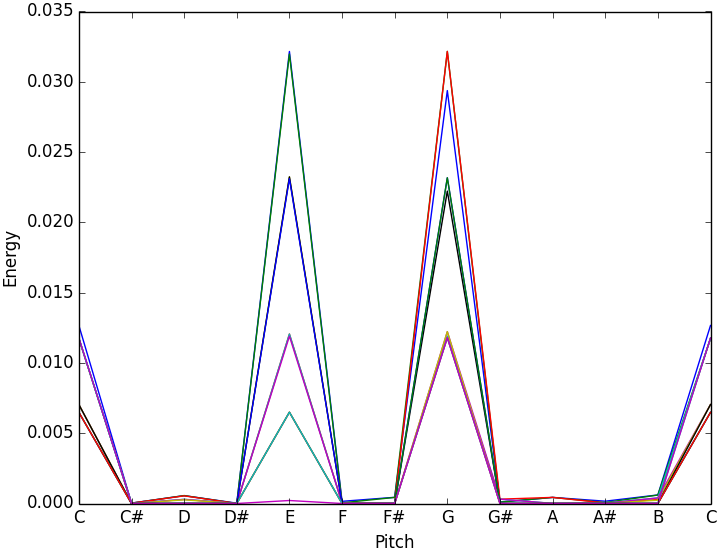
\includegraphics[width=\columnwidth]{chromac}}
\caption{Chroma features for Cmaj in various octaves and inversions}
\label{chroma}
\end{center}
\vskip -0.2in
\end{figure}

To test the performance of Chroma features against MFCC features, we start with
a binary classification problem of distinguishing major chords from minor
chords. An SVM with RBF kernel $$ K(x, z) = \exp(-\gamma\lVert{x - y}\rVert^2)$$
is trained, with regularization and kernel parameters ($\gamma = 1$ and $C =
100$). Table 1 summarizes the results, and confirms that chroma features are
much better suited to the task of chord recognition than MFCCs.

\begin{table}[t]
\caption{Accuracies for MFCC and Chroma on the binary classification task of
distinguishing between major and minor chords}
\label{mfccvschroma}
\vskip 0.15in
\begin{center}
\begin{small}
\begin{sc}
\begin{tabular}{lcccr}
\hline
\abovespace\belowspace
Features & Test Accuracy \\
\hline
\abovespace
MFCC & 51.0\%\\
Chroma & 97.7\%\\
\hline
\end{tabular}
\end{sc}
\end{small}
\end{center}
\vskip -0.1in
\end{table}

\section{Initial Models}
\subsection{Frame Model}
With Chroma established as good features for the chord recognition model, we can
now extend to the multiclass classification problem of determining the exact
chord. We first use multinomial logistic regression, also called softmax
regression, as our initial frame model. The frame model is responsible for
making predictions on individual frames. Table 2 shows the accuracies achieved
by the softmax classifier on the training and test set.
\begin{table}[t]
\caption{Softmax Regression frame model train and test accuracies}
\label{softmax}
\vskip 0.15in
\begin{center}
\begin{small}
\begin{sc}
\begin{tabular}{lcccr}
\hline
\abovespace\belowspace
Set & Accuracy \\
\hline
\abovespace
Traning & 51.2\%\\
Testing & 32.1\%\\
\hline
\end{tabular}
\end{sc}
\end{small}
\end{center}
\vskip -0.1in
\end{table}

\subsection{Mixer Model}
Our frame model outputs a prediction for each frame. Our final classification
task, however, is on an audio file, which consists of a sequence of f frames.
Let us first make the simplifying assumption that a test sound file consists of
a single chord being played.

We now define a mixer model, which is a model for collecting and using the
results on individuals frames outputted by the frame model. A simple mixer
model, the Middle Frame model, outputs the result for the entire file based on
the frame model's output for middle frame in the file. Another simple model, the
Max Count model, counts the most frequent prediction made across all of the
frames.

Consider another such model, we call the Independence Mixer model, which assumes
that the prediction on each frame is independent of the prediction on other
frames. The probability that chord y is the single chord played in the file is
calculated by considering the probability that y is the chord played at each
frame. For a test example, our predicted output is $y_p =
\underset{y}{\operatorname{argmax}} p(y | X) = p(y | x_1, x_2, ... x_f) =
\prod_{i=1}^fp(y | x_i)$.

Note that each $p(y | x_i)$ is given by our softmax frame model. The accuracies
achieved with different Mixer Models are summarized in Table 3.
\begin{figure}[ht]
\vskip 0.2in
\begin{center}
\centerline{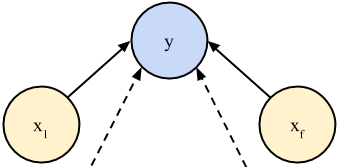
\includegraphics[width=\columnwidth]{naive}}
\caption{Bayesian network of Independence Mixer model}
\label{icml-historical}
\end{center}
\vskip -0.2in
\end{figure}

\begin{table}[t]
\caption{Comparisons of accuracies of mixer models with softmax frame model}
\label{mfccvschroma}
\vskip 0.15in
\begin{center}
\begin{small}
\begin{sc}
\begin{tabular}{lcccr}
\hline
\abovespace\belowspace
Model & Test Accuracy \\
\hline
\abovespace
Middle Frame & 6.7\%\\
Max Count & 33.3\%\\
Independence Mixer & 48.3\%\\
\hline
\end{tabular}
\end{sc}
\end{small}
\end{center}
\vskip -0.1in
\end{table}
\section{Improved Models}
\subsection{Improved Frame Model}

Softmax regression is a learning algorithm that models $p(y|x)$, the conditional
distribution of the chord given the extracted frame features. We now look at a
model that tries to model $p(x|y)$ and $p(y)$: Gaussian Discriminant Analysis
(GDA). \cite{jiang}. We model $p(x|y)$ using a multivariate normal distribution.
Although we model each gaussian with different means, we assume they all share
the same covariance matrix: $x|y=i \sim \mathcal{N}$$(\mu_i, \Sigma)$. Since our
aim is to make the system independent of any specific genre, we model $p(y) =
1/24$, a model in which all chords are equally likely. Table 4 summarizes the classification accuracies.

\begin{table}[t]
\caption{GDA frame model accuracies}
\label{mfccvschroma}
\vskip 0.15in
\begin{center}
\begin{small}
\begin{sc}
\begin{tabular}{lcccr}
\hline
\abovespace\belowspace
Set & Accuracy \\
\hline
\abovespace
Traning & 67.8\%\\
Testing & 53.9\%\\
\hline
\end{tabular}
\end{sc}
\end{small}
\end{center}
\vskip -0.1in
\end{table}


\subsection{Improved Mixer Model}
Earlier, we had imposed the constraint that chords could not change in a WAV
file. Our next model allows us to drop that constraint. We now use a Hidden
Markov Model to predict the chord sequence in sound files, allowing us to
determine chord changes in a file \cite{sheh}. Firstly, the emission
probabilities $p(x|y)$ are modelled by our GDA frame model. While state
transitions are usually learned in chord recognition tasks, \cite{lee}, since
each genre of music has a different distribution of transitions, assuming
uniform state transitions allows us to remain flexible to any genre of music. We
determine the most likely state sequence by the Viterbi decoding. Table 4
summarizes the accuracies acheived by the improved mixer model trained on
different sets of instruments.

Figure 3 shows the confusion matrix. The most common misclassifications are ones
between a major chords and its corresponding minor version. This is explained by
the fact that a major and a minor chord for any note have two out of three notes
in common.

\begin{figure}[ht]
\vskip 0.2in
\begin{center}
\centerline{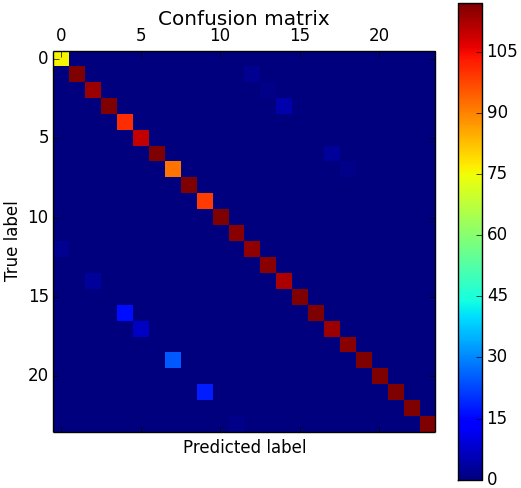
\includegraphics[width=\columnwidth]{conf}}
\caption{Confusion matrix for HMM training and testing on Piano}
\label{icml-historical}
\end{center}
\vskip -0.2in
\end{figure}

\begin{figure}[ht]
\vskip 0.2in
\begin{center}
\centerline{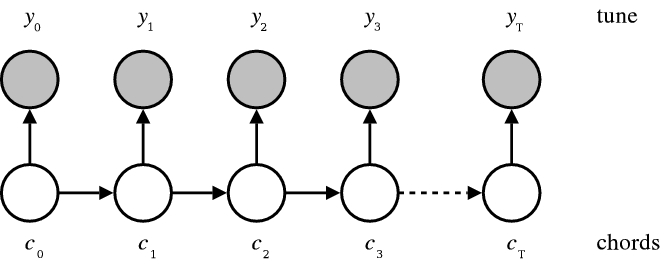
\includegraphics[width=\columnwidth]{hmm}}
\caption{Hidden Markov Model to determine most likely chord state sequences}
\label{icml-historical}
\end{center}
\vskip -0.2in
\end{figure}

\begin{table}[t]
\caption{HMM accuracies training and testing on different data sets}
\label{hmmacc}
\vskip 0.15in
\begin{center}
\begin{small}
\begin{sc}
\begin{tabular}{lcccr}
\hline
\abovespace\belowspace
Training Data & Testing Data & Accuracy \\
\hline
\abovespace
Piano & Piano & 97.01\%\\
Piano & Guitar & 99.46\%\\
Piano & Violin & 72.15\%\\
All & All & 90.68\%\\
\hline
\end{tabular}
\end{sc}
\end{small}
\end{center}
\vskip -0.1in
\end{table}

\section{Improving Features}

Chroma features, in their invariance to octave and inversions, make great
features for the chord recognition task. To boost the accuracy further would
require features were invariant of instruments \cite{jiang}. CRP (Chroma
DCT-Reduced log Pitch) is a chroma-based audio feature that boosts the degree of
timbre invariance. The general idea is to extract Chroma features, and then
discard timbre-related information similar to that expressed by MFCCs, in effect
leaving the information related to pitch. Table 5 summarizes the accuracies
achieved by the new CRP features in relation to the Chroma features.

\begin{figure}[ht]
\vskip 0.2in
\begin{center}
\centerline{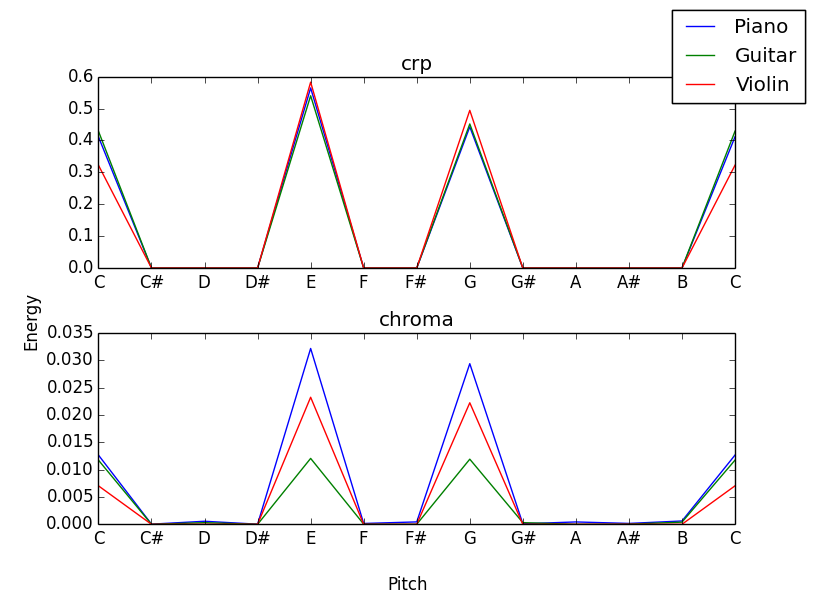
\includegraphics[width=\columnwidth]{chromacrp}}
\caption{CRP vs. Chroma Features for different instruments. Note the invariance of CRP to instruments.}
\label{icml-historical}
\end{center}
\vskip -0.2in
\end{figure}

\begin{table}[t]
\caption{Chroma vs CRP}
\label{chromavscrp}
\vskip 0.15in
\begin{center}
\begin{small}
\begin{sc}
\begin{tabular}{lcccr}
\hline
\abovespace\belowspace
Training Data & Testing Data & Accuracy \\
\hline
\abovespace
Piano & Piano & 98.72\%\\
Piano & Guitar & 99.96\%\\
Piano & Violin & 98.54\%\\
All & All & 99.19\%\\
\hline
\end{tabular}
\end{sc}
\end{small}
\end{center}
\vskip -0.1in
\end{table}

\section{Live System Considerations}

A live system presents new challenges for chord recognition, while pushing the
extents of possible uses of the system.
One of the most important considerations for a live system to take into account
is noise. It is important for a system to not predict any chord in this
timespan.

Our realtime system makes use of the Web Audio API to capture live audio. Every
800ms, we encode the audio in WAV format, and transfer it to a server using
WebSockets. We then extract features for every 100ms frame in the WAV file, and
predict the most likely chord sequence in the 800ms using the HMM.

\subsection{Handling Noise}
At this stage, we are able to determine whether the 800ms segment is a noise or
a chord. Using the knowledge that it usually takes a few seconds before chords
change, we can then post-process the output by looking at the number of times
chord changes were predicted by the HMM in the 800ms segment. If any chord lasts
for more than 400ms in the prediction, then we output the chord as our
prediction for the 800ms segment. Otherwise, we understand that segment of sound
as consisting of noise.

\subsection{Recording Interval}
We found 800ms to be the optimal time interval over which to process the audio. Increasing the interval 
for collecting the recording from 800ms was found to create a noticeable delay in the live system. On the other hand, reducing the window time not only decreased accuracy, but also made it harder to distinguish between noise and chords.

\section{Conclusion}
In this paper, we present an implementation of a real-time chord recognition system. We show the effectiveness of Hidden Markov Models with Gaussian emissions in classifying chords. Furthermore, we show how timbre-invariant CRP features can improve robustness, compared to Chroma. Integrating noise detection strategies then creates an effective live recognition system.
that could be start of conclusion, at least a closing sentence?


\bibliography{example_paper}
\bibliographystyle{icml2013}

\end{document}
